% ==============================================================================
% 3.5 IMPLEMENTACIÓN (flujo de trabajo PUDS dentro del Capítulo 3)
% Reutiliza el cap. 8 de main.tex (secciones/10_capitulo8_implementacion/).
% Los encabezados 8.x se muestran como 3.5.x mediante \wfa, \wfb y \wn{8}.
% ==============================================================================
\subsection{3.5. Implementación}\label{sec:v2_implementacion}

Este flujo de trabajo del PUDS describe cómo quedó construido el sistema a partir del código desarrollado: la arquitectura del sistema, la arquitectura de cada subsistema y las herramientas utilizadas. Los estándares de codificación y de comentarios aplicados se definen en la sección 2.12 del Capítulo 2.

% ------------------------------------------------------------------------------
% 8.1. IMPLEMENTACIÓN DE LA ARQUITECTURA DEL SISTEMA
% ------------------------------------------------------------------------------
\wfa{\wn{8}.1. Implementación de la Arquitectura del Sistema}\label{sec:cap8_arquitectura_sistema}

Este capítulo describe cómo quedó construido el sistema ComedorUAGRM a partir del código desarrollado. La arquitectura diseñada en el capítulo 7 se conserva: clientes web y móvil, una API REST en Spring Boot organizada en seis paquetes funcionales, un módulo de preselección en Python y una base de datos PostgreSQL. Los diagramas de componentes del capítulo se elaboraron en Sparx Enterprise Architect y reflejan las clases reales del código.

El sistema se implementó como una aplicación cliente-servidor en capas, desplegada con Docker Compose. Los clientes son el panel web (React y TypeScript), la aplicación móvil (Flutter) y la landing institucional de Nexware (Astro). El tráfico HTTP del navegador pasa por un proxy inverso nginx que sirve el panel en la raíz, la landing en \texttt{/landing-page} y la API en \texttt{/api/}. El software central es la API REST \texttt{comedor-uagrm-core} (Java 21 y Spring Boot 4.1), organizada en los seis subsistemas definidos en el análisis. Esta API consume el módulo de IA \texttt{comedor-uagrm-ia} (Python y FastAPI), accesible solo desde ella por la red interna, y los servicios externos de correo (SMTP) y Firebase Cloud Messaging.

Los datos residen en PostgreSQL 18, con una base transaccional (OLTP) de 31 tablas gestionada con migraciones Flyway. El tablero de indicadores BI no usa un almacén OLAP ni cubos: se alimenta de cinco vistas materializadas de la misma base (\texttt{mv\_indicadores\_convocatoria}, \texttt{mv\_bi\_convocatoria}, \texttt{mv\_bi\_asistencia\_dia}, \texttt{mv\_bi\_carrera\_convocatoria} y \texttt{mv\_bi\_puntaje\_convocatoria}), que se refrescan periódicamente. Los archivos (documentos adjuntos, actas y planillas en PDF) se almacenan en MinIO, compatible con S3. Redis se emplea como caché únicamente en el caso de uso CU12 (dashboard de indicadores BI).

La Figura~\ref{fig:impl_sistema} presenta el diagrama de componentes del sistema completo: los seis paquetes de subsistemas con los casos de uso que los conforman, el software central, la base de datos transaccional (OLTP), las vistas de indicadores BI, el módulo de IA, MinIO y Redis. Los paquetes se relacionan según el flujo del proceso: becados y asistencia utiliza auditoría y adjudicación, esta utiliza convocatoria y postulación, y esta última utiliza preselección con IA. La Tabla~\ref{tab:impl_subsistemas} resume los casos de uso de cada subsistema.

\begin{table}[H]
\caption{Subsistemas y casos de uso que los conforman}
\label{tab:impl_subsistemas}
\centering
\footnotesize\linespread{1}\selectfont
\renewcommand{\arraystretch}{1.3}
\begin{tabular}{>{\raggedright\arraybackslash}p{5.5cm}>{\raggedright\arraybackslash}p{9.5cm}}
\toprule
\textbf{Subsistema} & \textbf{Casos de uso} \\
\midrule
Cuentas y Acceso & CU01, CU14, CU15 \\
Convocatoria y Postulación & CU13, CU02, CU16, CU17, CU18, CU04 \\
Preselección con IA & CU03, CU26 \\
Auditoría y Adjudicación & CU05, CU06, CU07, CU08, CU19, CU20, CU21, CU22 y el servicio de notificaciones (CU-EXTRA-01) \\
Becados y Asistencia & CU23, CU09, CU10, CU11, CU24 \\
Reportes y Trazabilidad & CU12, CU25 \\
\bottomrule
\end{tabular}

\smallskip
\noindent\raggedright\textit{Nota.} Elaboración propia.
\end{table}

\begin{landscape}
\begin{figure}[p]
\caption{Diagrama de Componentes de la Implementación de la Arquitectura del Sistema}
\label{fig:impl_sistema}
\centering
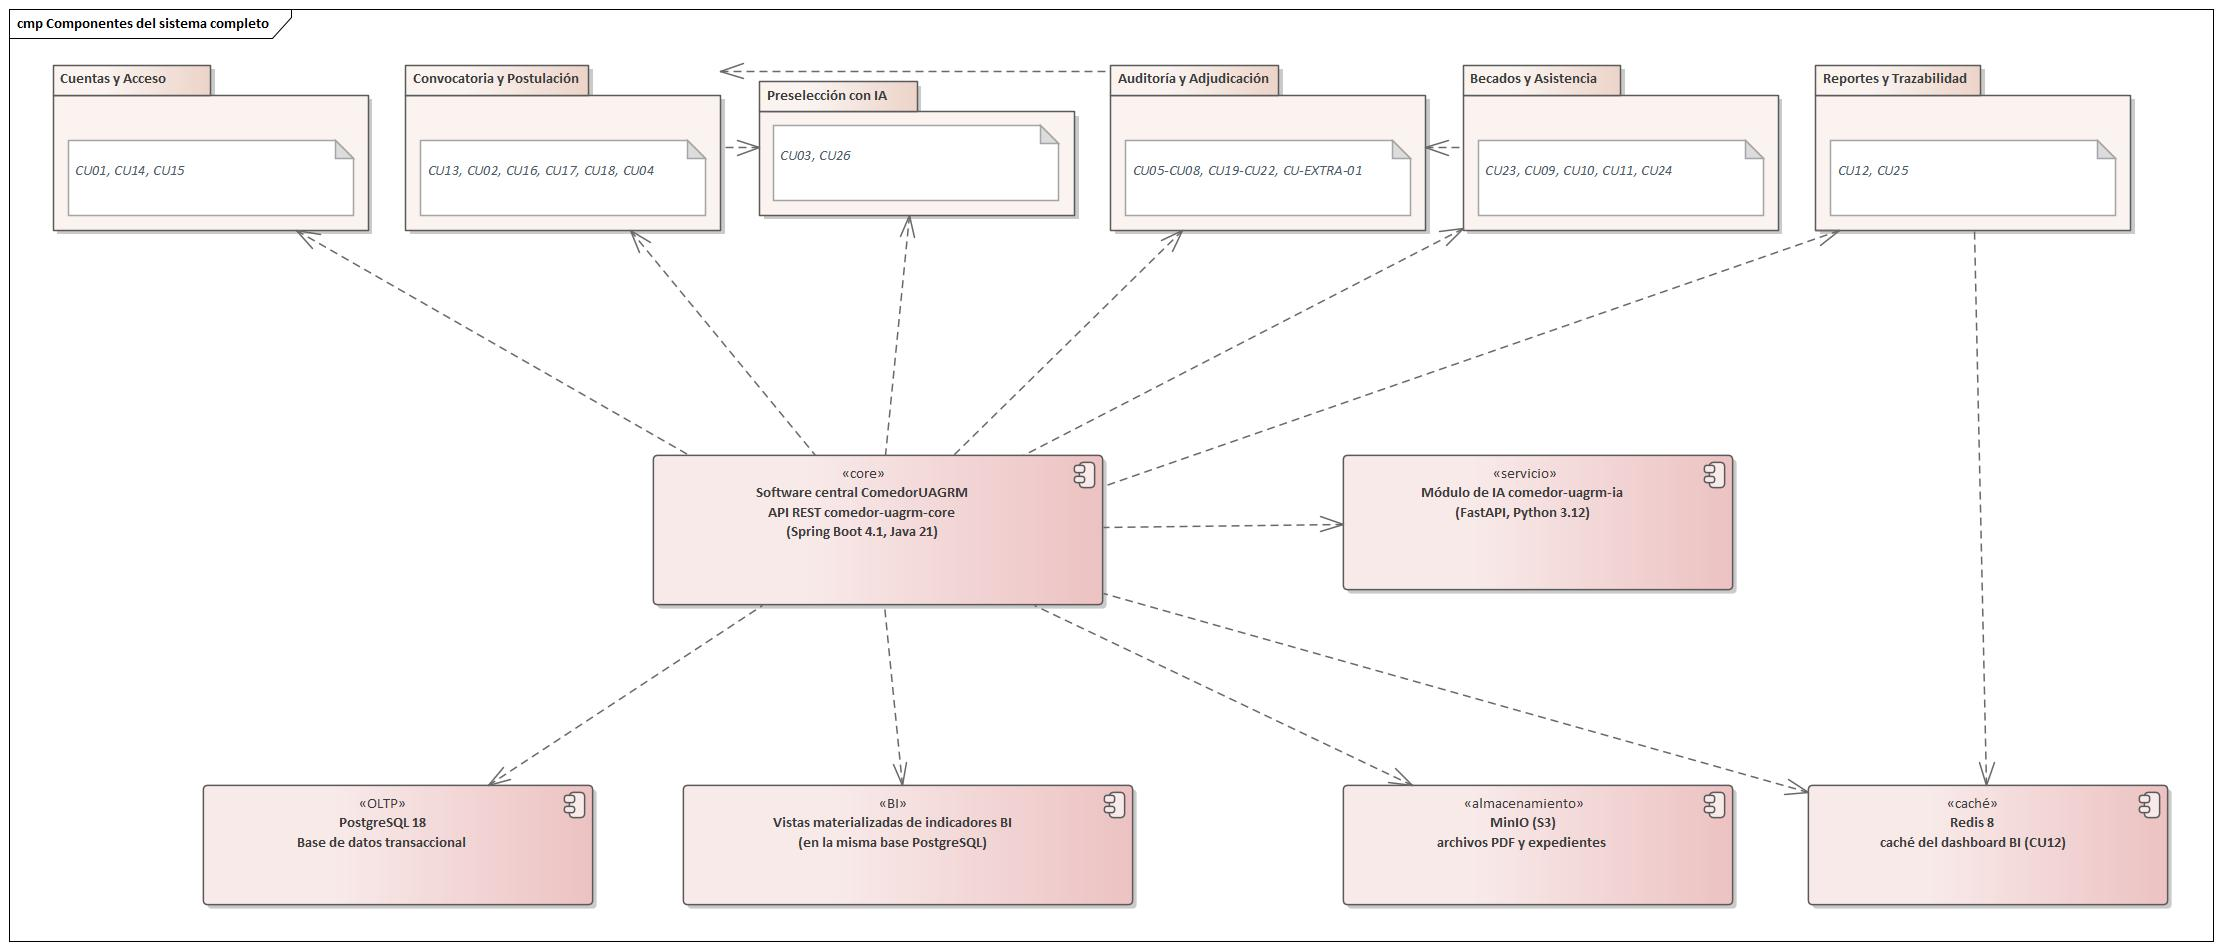
\includegraphics[width=\linewidth,height=0.8\textheight,keepaspectratio]{images/147_Componentes_Sistema_Completo.jpg}

\smallskip
\noindent\raggedright\textit{Nota.} Elaboración propia.
\end{figure}
\end{landscape}


% ------------------------------------------------------------------------------
% 8.2. IMPLEMENTACIÓN DE LA ARQUITECTURA DEL SUBSISTEMA
% ------------------------------------------------------------------------------
\wfa{\wn{8}.2. Implementación de la Arquitectura del Subsistema}\label{sec:cap8_arquitectura_subsistema}

Cada subsistema sigue la misma arquitectura en tres capas, que corresponde a la organización por \textit{features} del código. La capa de cliente contiene las pantallas del panel web (una carpeta por \textit{feature} en React) y, cuando el caso de uso lo requiere, las pantallas y servicios de la aplicación móvil. La capa de servicio y negocio está en el paquete \texttt{com.comedoruagrm.backend.features} de Spring Boot: los controladores REST validan la entrada y delegan en servicios; los servicios contienen la lógica, las transacciones y la auditoría; y los repositorios, interfaces de Spring Data JPA o consultas SQL directas, acceden a la base de datos. La capa de base de datos corresponde a las tablas de PostgreSQL de cada paquete funcional. Las flechas de los diagramas indican dependencia de uso y se obtuvieron de las dependencias inyectadas en el código; para no recargar los diagramas, no se dibujan las lecturas de apoyo a tablas de otros subsistemas.


\wfb{\wn{8}.2.1. Implementación de la Arquitectura del Subsistema Cuentas y Acceso}\label{sec:cap8_sub_p1}

Este subsistema agrupa los casos de uso CU01, CU14, CU15.

Gestiona las cuentas del sistema: registro e inicio de sesión con JWT propio (token de acceso de 15 minutos y \textit{refresh token} de 7 días, enviados en cookies \texttt{HttpOnly} en la web y como \textit{Bearer} en móvil), recuperación y cambio de contraseña mediante un enlace enviado por correo, perfil del usuario y administración de las cuentas del personal y sus roles. Los controladores delegan en los servicios del subsistema; la sesión se guarda en la tabla \texttt{sesion} solo como hash del \textit{refresh token}.

La Figura~\ref{fig:impl_p1} presenta el diagrama de componentes del subsistema. Sus componentes son los siguientes:

\begin{itemize}
\item \textbf{Cliente web:} \texttt{LoginScreen}, \texttt{RegistroScreen}, \texttt{RecuperarContrasenaScreen}, \texttt{RestablecerContrasenaScreen}, \texttt{PerfilScreen}, \texttt{UsuariosPersonalScreen}.
\item \textbf{Cliente móvil:} \texttt{login\_screen}, \texttt{registro\_screen}, \texttt{recuperar\_contrasena\_screen}, \texttt{perfil\_screen}.
\item \textbf{Controladores:} \texttt{AuthController}, \texttt{UsuarioController}, \texttt{PerfilController}, \texttt{CarreraController}.
\item \textbf{Servicios:} \texttt{AuthService}, \texttt{SesionService}, \texttt{RestablecimientoContrasenaService}, \texttt{CorreoRestablecimientoService}, \texttt{UsuarioService}, \texttt{UsuarioPersonalService}, \texttt{PerfilService}, \texttt{CarreraService}.
\item \textbf{Repositorios:} \texttt{SesionRepository}, \texttt{UsuarioRepository}, \texttt{PostulanteRepository}, \texttt{RolRepository}, \texttt{CarreraRepository}.
\item \textbf{Tablas:} \texttt{sesion}, \texttt{usuario}, \texttt{postulante}, \texttt{rol}, \texttt{carrera}.
\item \textbf{Componentes externos:} Servicio de correo (SMTP).
\end{itemize}

\begin{landscape}
\begin{figure}[p]
\caption{Diagrama de Componentes de la Implementación de la Arquitectura del Subsistema Cuentas y Acceso}
\label{fig:impl_p1}
\centering
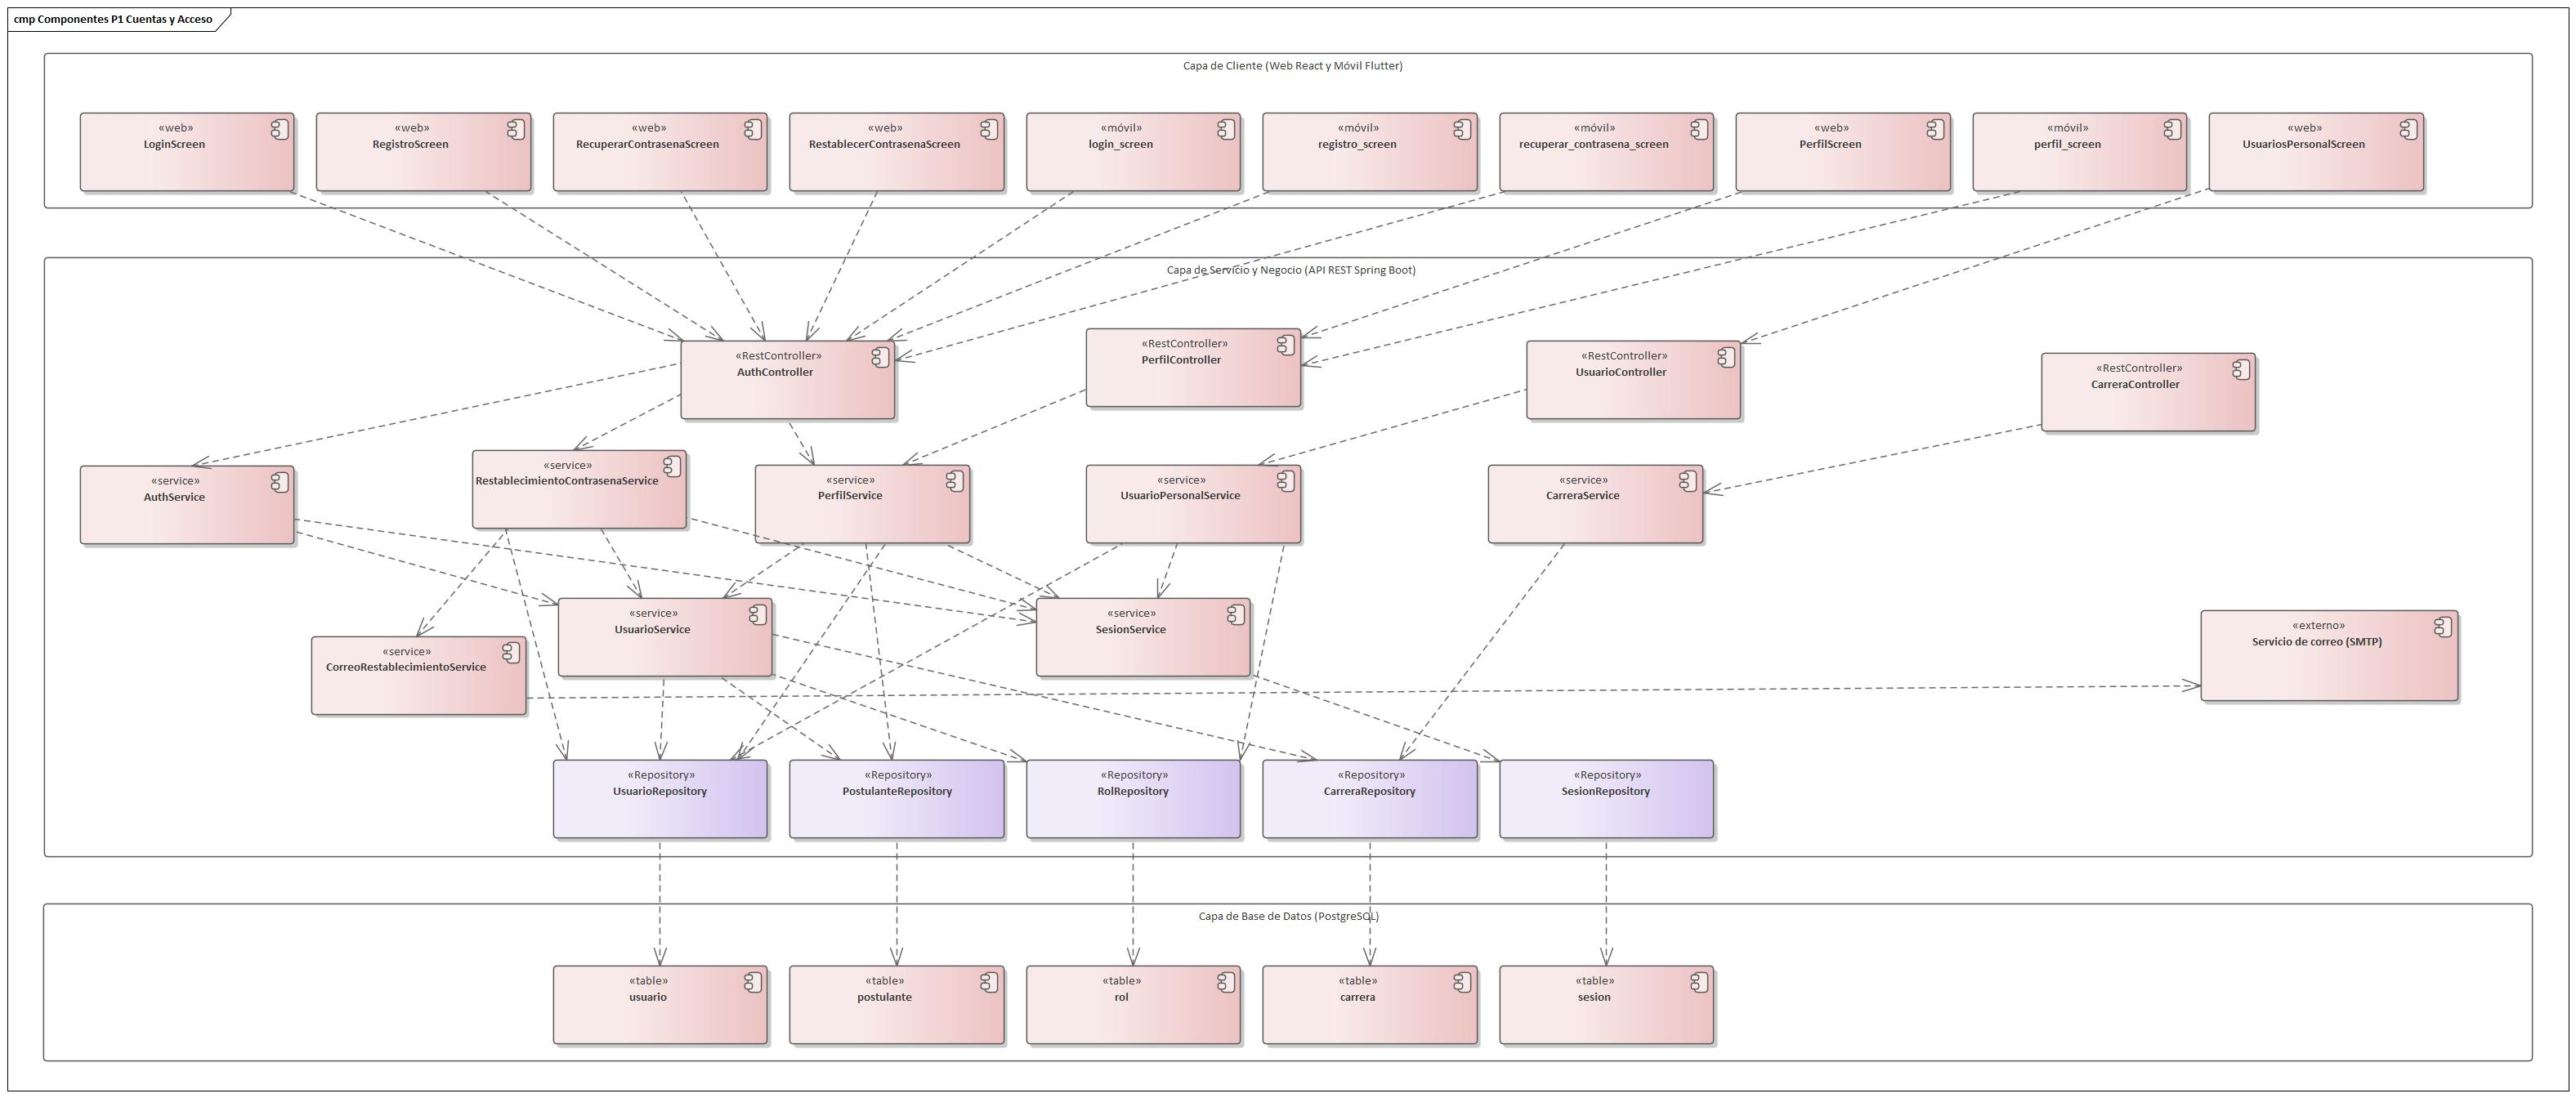
\includegraphics[width=\linewidth,height=0.8\textheight,keepaspectratio]{images/148_Componentes_P1_Cuentas_y_Acceso.jpg}

\smallskip
\noindent\raggedright\textit{Nota.} Elaboración propia.
\end{figure}
\end{landscape}


\wfb{\wn{8}.2.2. Implementación de la Arquitectura del Subsistema Convocatoria y Postulación}\label{sec:cap8_sub_p2}

Este subsistema agrupa los casos de uso CU13, CU02, CU16, CU17, CU18, CU04.

Cubre la apertura y cierre de convocatorias y gestiones académicas, y la postulación del estudiante: guardar el borrador, adjuntar documentos (almacenados en MinIO), validar elegibilidad y duplicados, enviar la postulación y consultar su estado. \texttt{CierreAutomaticoConvocatoriasJob} cierra las convocatorias vencidas. Al enviar la postulación, \texttt{EnvioPostulacionService} dispara la precalificación del subsistema de preselección con IA.

La Figura~\ref{fig:impl_p2} presenta el diagrama de componentes del subsistema. Sus componentes son los siguientes:

\begin{itemize}
\item \textbf{Cliente web:} \texttt{ConvocatoriasScreen}, \texttt{GestionesAcademicasScreen}, \texttt{PostularScreen}, \texttt{MisPostulacionesScreen}, \texttt{DetallePostulacionScreen}, \texttt{DocumentosPostulacionScreen}.
\item \textbf{Cliente móvil:} \texttt{postular\_screen}, \texttt{detalle\_postulacion\_screen}, \texttt{documentos\_postulacion\_screen}, \texttt{revisar\_documento\_screen}.
\item \textbf{Controladores:} \texttt{ConvocatoriaController}, \texttt{GestionAcademicaController}, \texttt{TipoDocumentoController}, \texttt{EnvioPostulacionController}, \texttt{BorradorPostulacionController}, \texttt{DocumentosPostulacionController}, \texttt{MisPostulacionesController}.
\item \textbf{Servicios:} \texttt{ConvocatoriaService}, \texttt{ConvocatoriaEstadoService}, \texttt{GestionAcademicaService}, \texttt{TipoDocumentoService}, \texttt{DocumentosConvocatoriaService}, \texttt{CierreAutomaticoConvocatoriasJob}, \texttt{EnvioPostulacionService}, \texttt{BorradorPostulacionService}, \texttt{DocumentosPostulacionService}, \texttt{ValidacionPostulacionService}, \texttt{MisPostulacionesService}.
\item \textbf{Repositorios:} \texttt{ConvocatoriaRepository}, \texttt{ConvocatoriaDocumentoRepository}, \texttt{GestionAcademicaRepository}, \texttt{TipoDocumentoRepository}, \texttt{PostulacionRepository}, \texttt{DocumentoAdjuntoRepository}, \texttt{PostulacionHistorialRepository}.
\item \textbf{Tablas:} \texttt{convocatoria}, \texttt{convocatoria\_documento}, \texttt{gestion\_academica}, \texttt{tipo\_documento}, \texttt{postulacion}, \texttt{documento\_adjunto}, \texttt{postulacion\_historial}.
\item \textbf{Componentes externos:} MinIO (archivos), Módulo de IA (FastAPI).
\end{itemize}

\begin{landscape}
\begin{figure}[p]
\caption{Diagrama de Componentes de la Implementación de la Arquitectura del Subsistema Convocatoria y Postulación}
\label{fig:impl_p2}
\centering
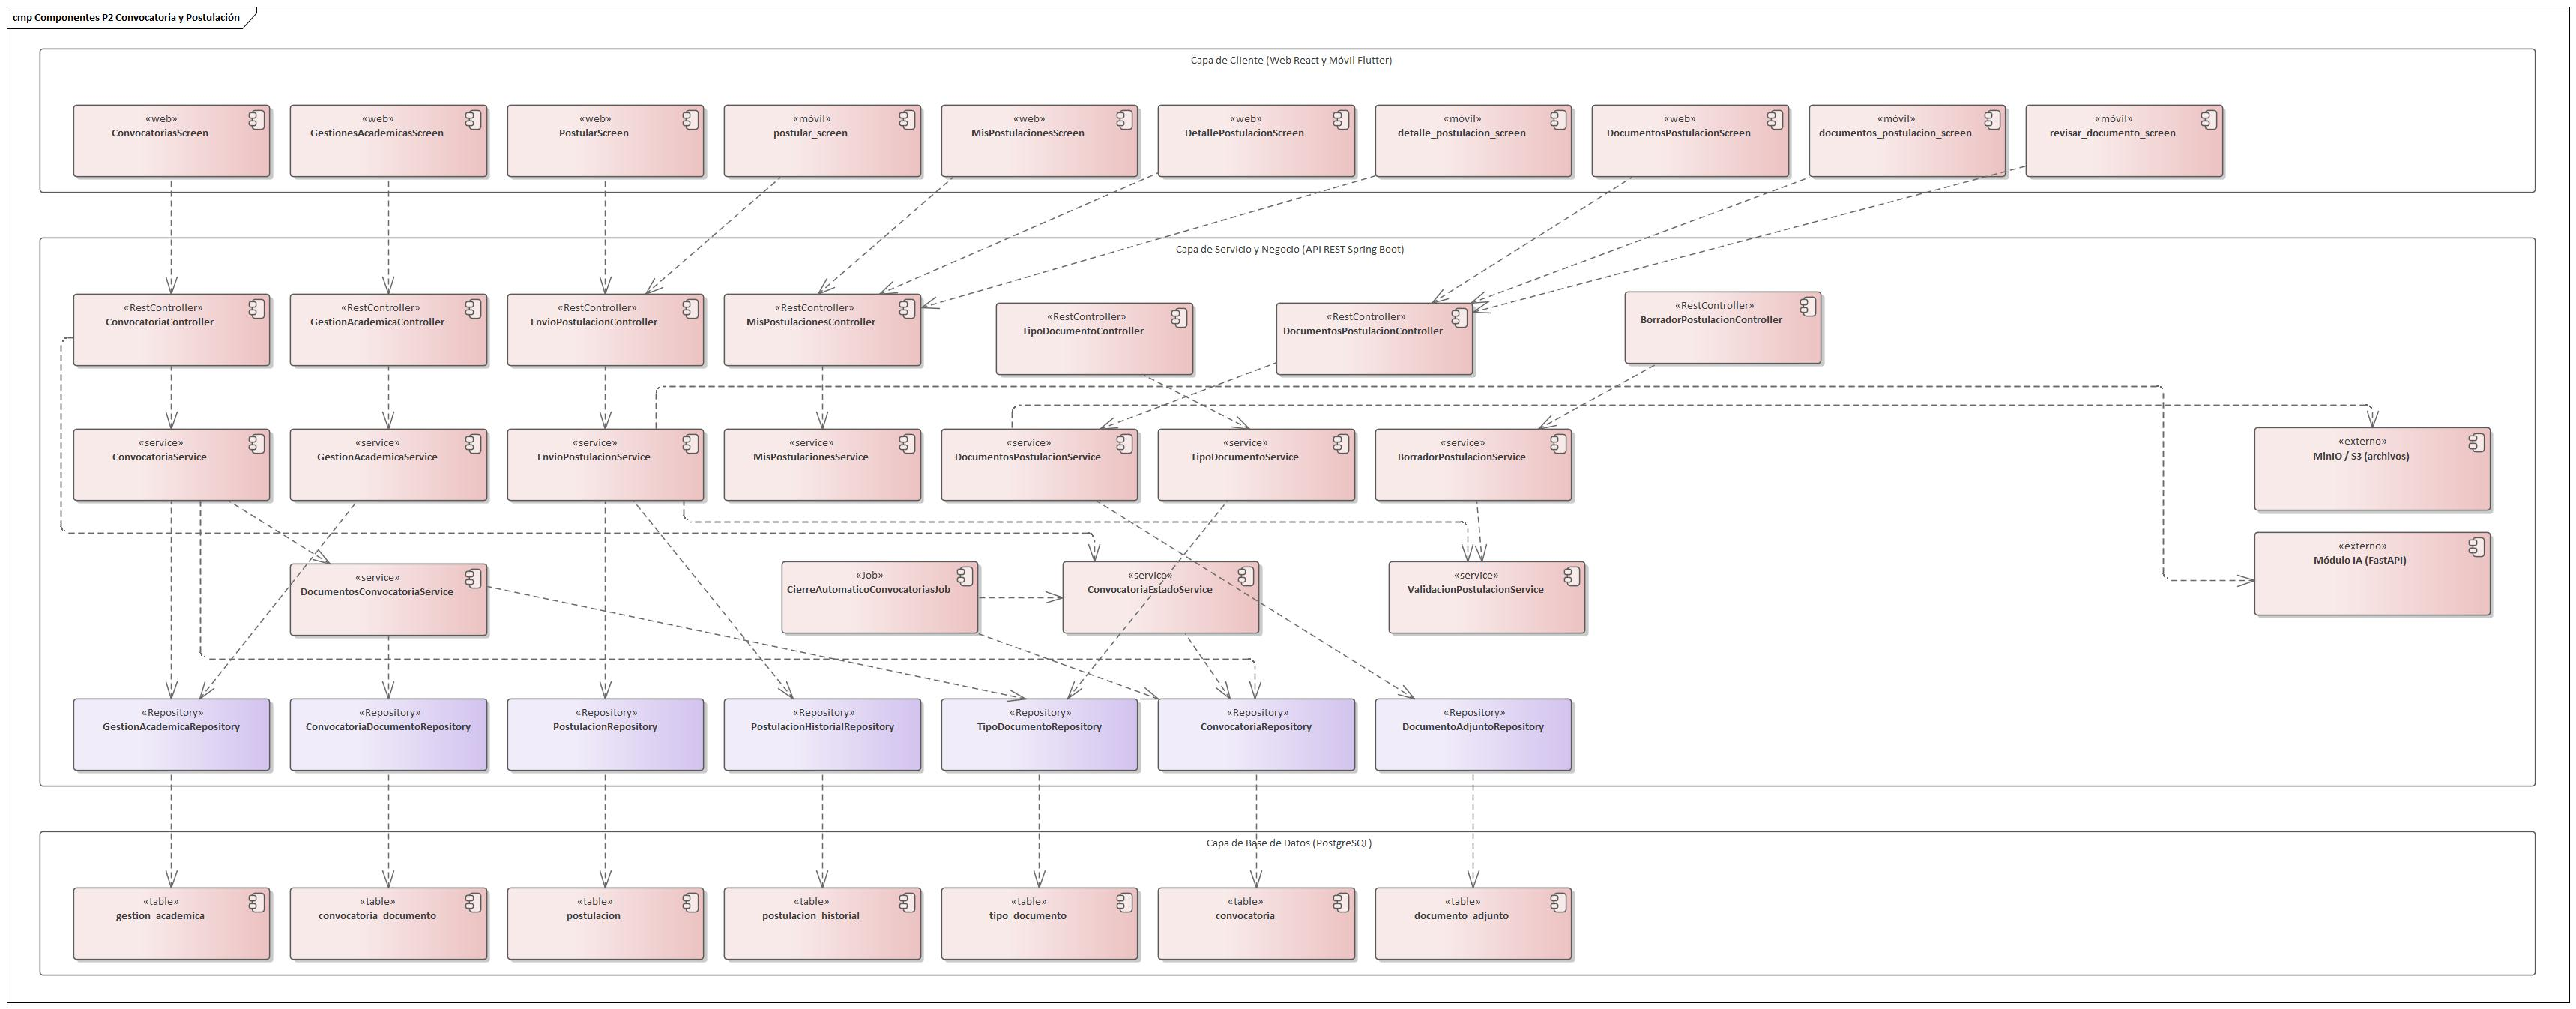
\includegraphics[width=\linewidth,height=0.8\textheight,keepaspectratio]{images/149_Componentes_P2_Convocatoria_y_Postulacion.jpg}

\smallskip
\noindent\raggedright\textit{Nota.} Elaboración propia.
\end{figure}
\end{landscape}


\wfb{\wn{8}.2.3. Implementación de la Arquitectura del Subsistema Preselección con IA}\label{sec:cap8_sub_p3}

Este subsistema agrupa los casos de uso CU03, CU26.

Calcula el puntaje de vulnerabilidad de cada postulación y permite a la DUBSS parametrizar el modelo y reprocesar los puntajes. \texttt{PrecalificacionClient} es la interfaz que abstrae al módulo de IA e \texttt{IaHttpPrecalificacionClient} la implementa llamando por HTTP interno a \texttt{POST /api/v1/puntaje} del módulo \texttt{comedor-uagrm-ia} (FastAPI); \texttt{PrecalificacionReintentoJob} reintenta las precalificaciones que fallaron. Los repositorios \texttt{ModeloPreseleccionConsultaRepository} y \texttt{ReprocesamientoConsultaRepository} acceden con SQL directo a \texttt{parametro\_modelo} y \texttt{lote\_reprocesamiento}.

La Figura~\ref{fig:impl_p3} presenta el diagrama de componentes del subsistema. Sus componentes son los siguientes:

\begin{itemize}
\item \textbf{Cliente web:} \texttt{PrecalificacionScreen}, \texttt{ParametrosModeloScreen}.
\item \textbf{Controladores:} \texttt{PrecalificacionController}, \texttt{ModeloPreseleccionController}, \texttt{ReprocesamientoController}.
\item \textbf{Servicios:} \texttt{PrecalificacionService}, \texttt{PrecalificacionDetalleService}, \texttt{IaHttpPrecalificacionClient}, \texttt{PrecalificacionReintentoJob}, \texttt{ModeloPreseleccionService}, \texttt{ReprocesamientoService}, \texttt{ReprocesamientoEjecucionService}.
\item \textbf{Repositorios:} \texttt{ModeloPreseleccionRepository}, \texttt{ModeloPreseleccionConsultaRepository}, \texttt{PuntajePostulacionRepository}, \texttt{ReprocesamientoConsultaRepository}.
\item \textbf{Tablas:} \texttt{modelo\_preseleccion}, \texttt{parametro\_modelo}, \texttt{puntaje\_postulacion}, \texttt{lote\_reprocesamiento}.
\item \textbf{Componentes externos:} Módulo de IA (FastAPI).
\end{itemize}

\begin{landscape}
\begin{figure}[p]
\caption{Diagrama de Componentes de la Implementación de la Arquitectura del Subsistema Preselección con IA}
\label{fig:impl_p3}
\centering
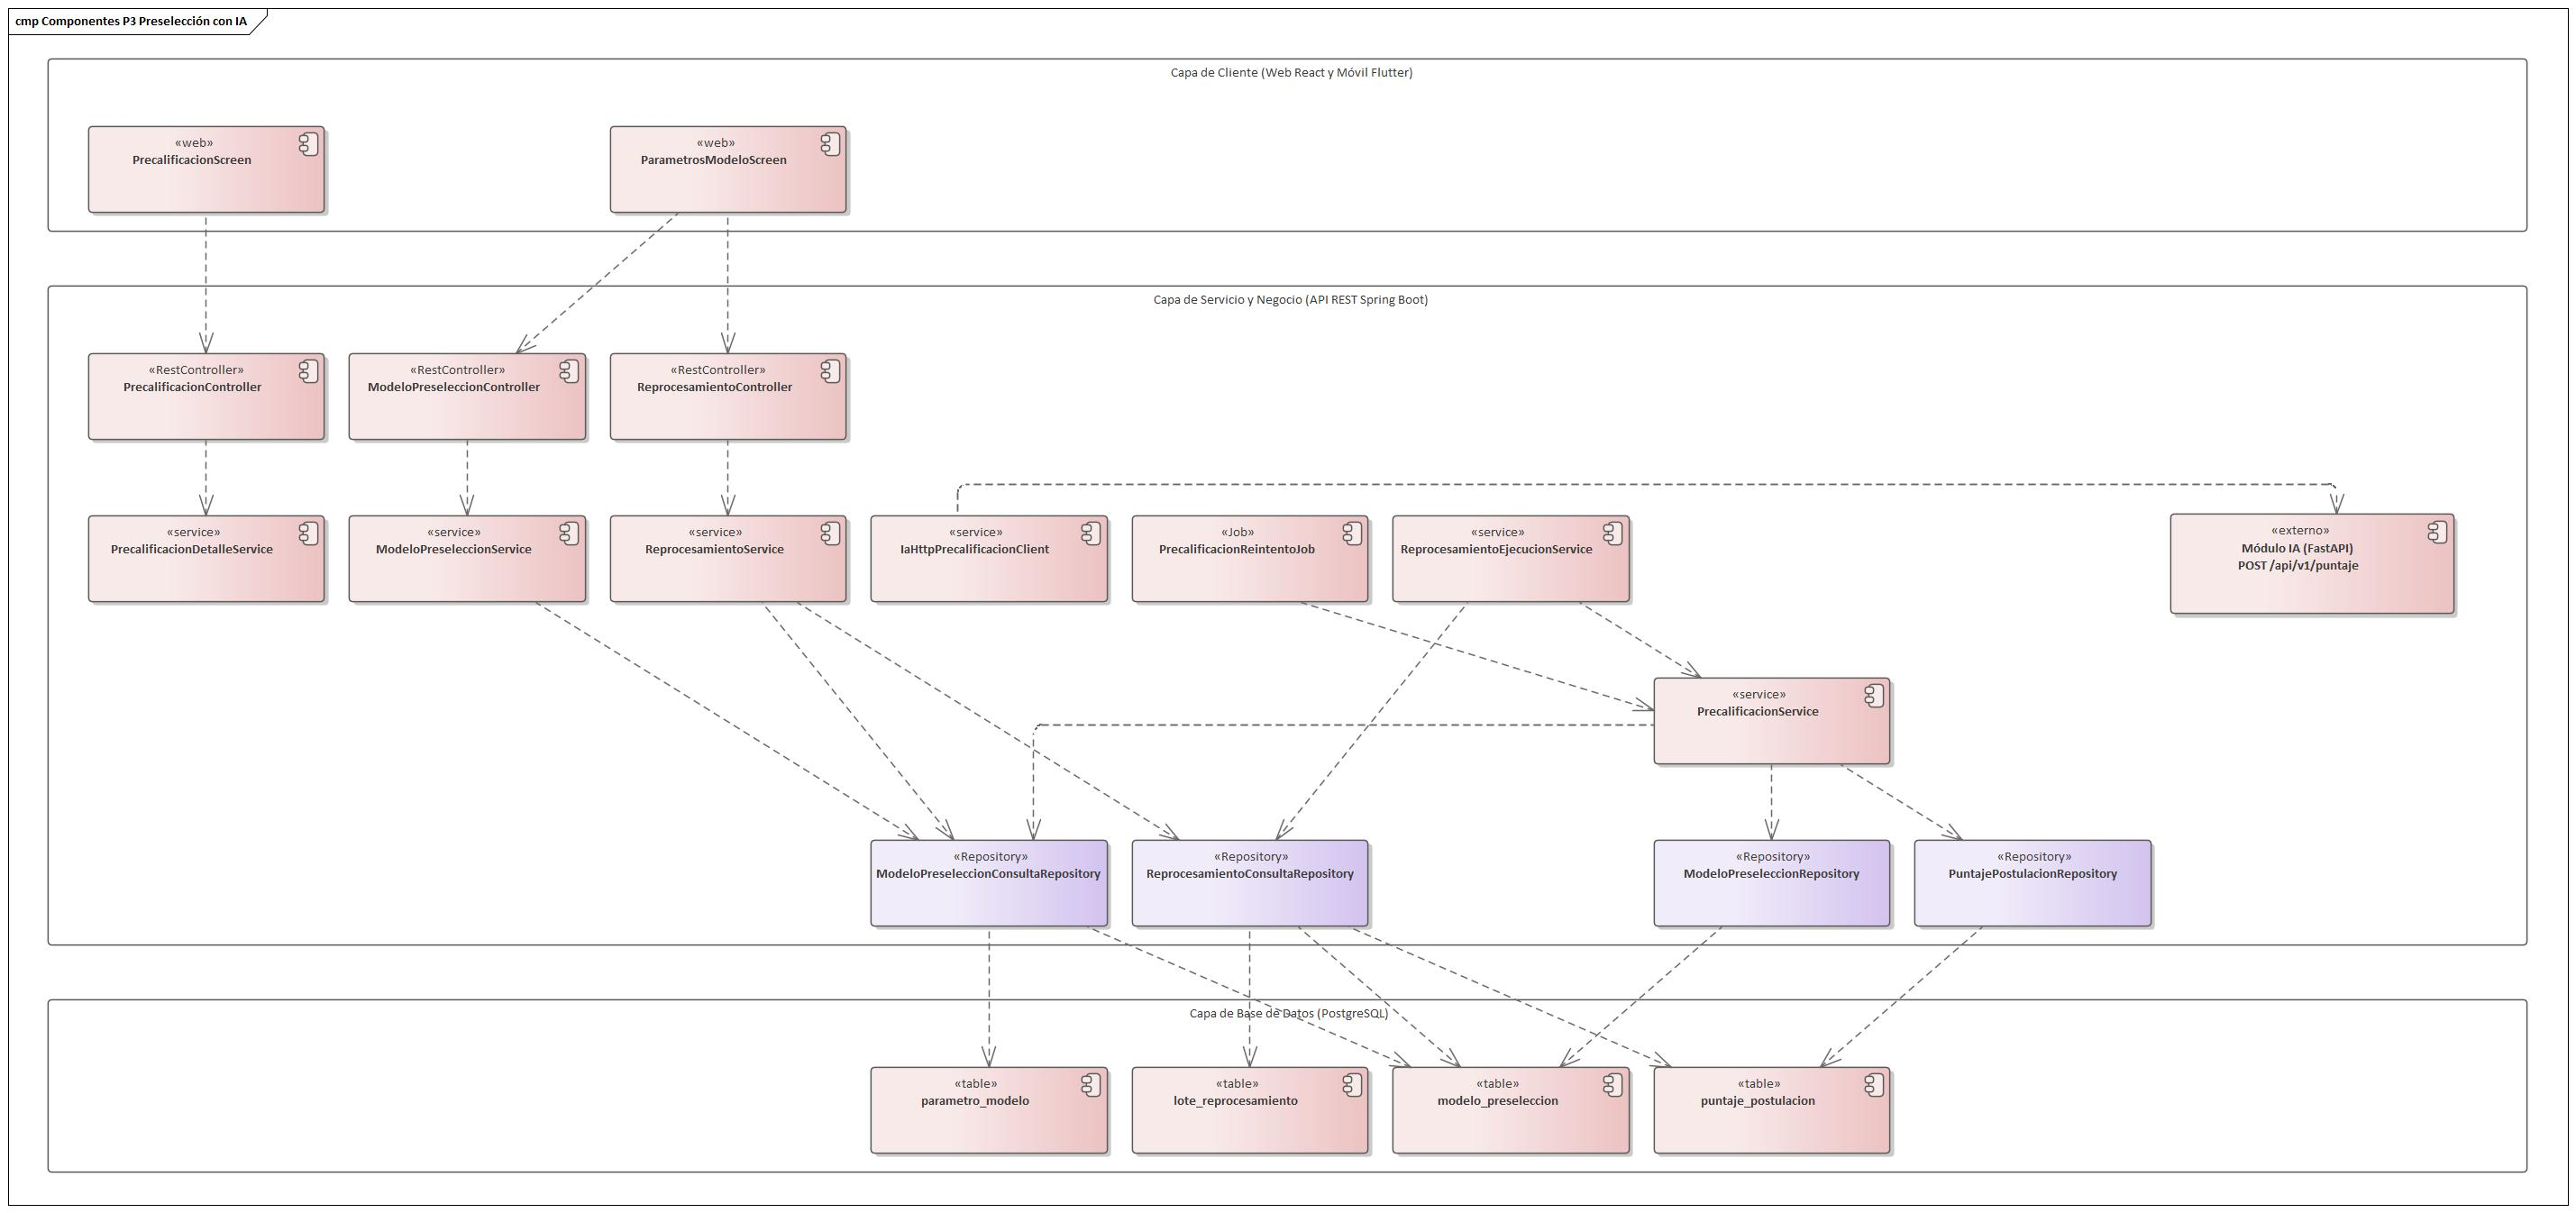
\includegraphics[width=\linewidth,height=0.8\textheight,keepaspectratio]{images/150_Componentes_P3_Preseleccion_IA.jpg}

\smallskip
\noindent\raggedright\textit{Nota.} Elaboración propia.
\end{figure}
\end{landscape}


\wfb{\wn{8}.2.4. Implementación de la Arquitectura del Subsistema Auditoría y Adjudicación}\label{sec:cap8_sub_p4}

Este subsistema agrupa los casos de uso CU05, CU06, CU07, CU08, CU19, CU20, CU21, CU22 y CU-EXTRA-01.

Concentra el proceso de la DUBSS sobre las postulaciones mejor puntuadas: lista priorizada, selección y notificación de finalistas, auditoría del expediente, devolución, archivo o rechazo, adjudicación, acta de adjudicación en PDF, comunicados y publicación de resultados. También contiene el servicio transversal de notificaciones (bandeja, correo y \textit{push} con Firebase Cloud Messaging) y el registro de dispositivos móviles.

La Figura~\ref{fig:impl_p4} presenta el diagrama de componentes del subsistema. Sus componentes son los siguientes:

\begin{itemize}
\item \textbf{Cliente web:} \texttt{ListaPriorizadaScreen}, \texttt{FinalistasScreen}, \texttt{ExpedienteScreen}, \texttt{AdjudicacionScreen}, \texttt{ActasScreen}, \texttt{PublicarResultadosScreen}, \texttt{ResultadosScreen}.
\item \textbf{Cliente móvil:} \texttt{firebase\_push\_service}.
\item \textbf{Controladores:} \texttt{ListaPriorizadaController}, \texttt{SeleccionFinalistasController}, \texttt{FinalistaController}, \texttt{ExpedienteController}, \texttt{DevolucionController}, \texttt{CierrePostulacionController}, \texttt{AdjudicacionController}, \texttt{ActaController}, \texttt{ComunicadoController}, \texttt{ResultadosAdminController}, \texttt{ResultadosPostulanteController}, \texttt{NotificacionController}, \texttt{DispositivoFcmController}.
\item \textbf{Servicios:} \texttt{ListaPriorizadaService}, \texttt{SeleccionFinalistasService}, \texttt{FinalistaService}, \texttt{ExpedienteService}, \texttt{DevolucionService}, \texttt{CierrePostulacionService}, \texttt{AdjudicacionService}, \texttt{ActaAdjudicacionService}, \texttt{ActaPdfService}, \texttt{ComunicadoService}, \texttt{PublicacionResultadosService}, \texttt{ResultadosAdminService}, \texttt{ResultadosPostulanteService}, \texttt{NotificacionService}, \texttt{DispositivoFcmService}.
\item \textbf{Repositorios:} \texttt{ListaPriorizadaRepository}, \texttt{FinalistaRepository}, \texttt{AuditoriaExpedienteRepository}, \texttt{AdjudicacionRepository}, \texttt{ActaAdjudicacionRepository}, \texttt{PublicacionResultadoRepository}, \texttt{ComunicadoRepository}, \texttt{NotificacionRepository}, \texttt{DispositivoFcmRepository}.
\item \textbf{Tablas:} \texttt{finalista}, \texttt{auditoria\_expediente}, \texttt{adjudicacion}, \texttt{acta\_adjudicacion}, \texttt{publicacion\_resultado}, \texttt{comunicado}, \texttt{notificacion}, \texttt{dispositivo\_fcm}.
\item \textbf{Componentes externos:} MinIO (actas y expedientes), Firebase Cloud Messaging, Servicio de correo (SMTP).
\end{itemize}

\begin{landscape}
\begin{figure}[p]
\caption{Diagrama de Componentes de la Implementación de la Arquitectura del Subsistema Auditoría y Adjudicación}
\label{fig:impl_p4}
\centering
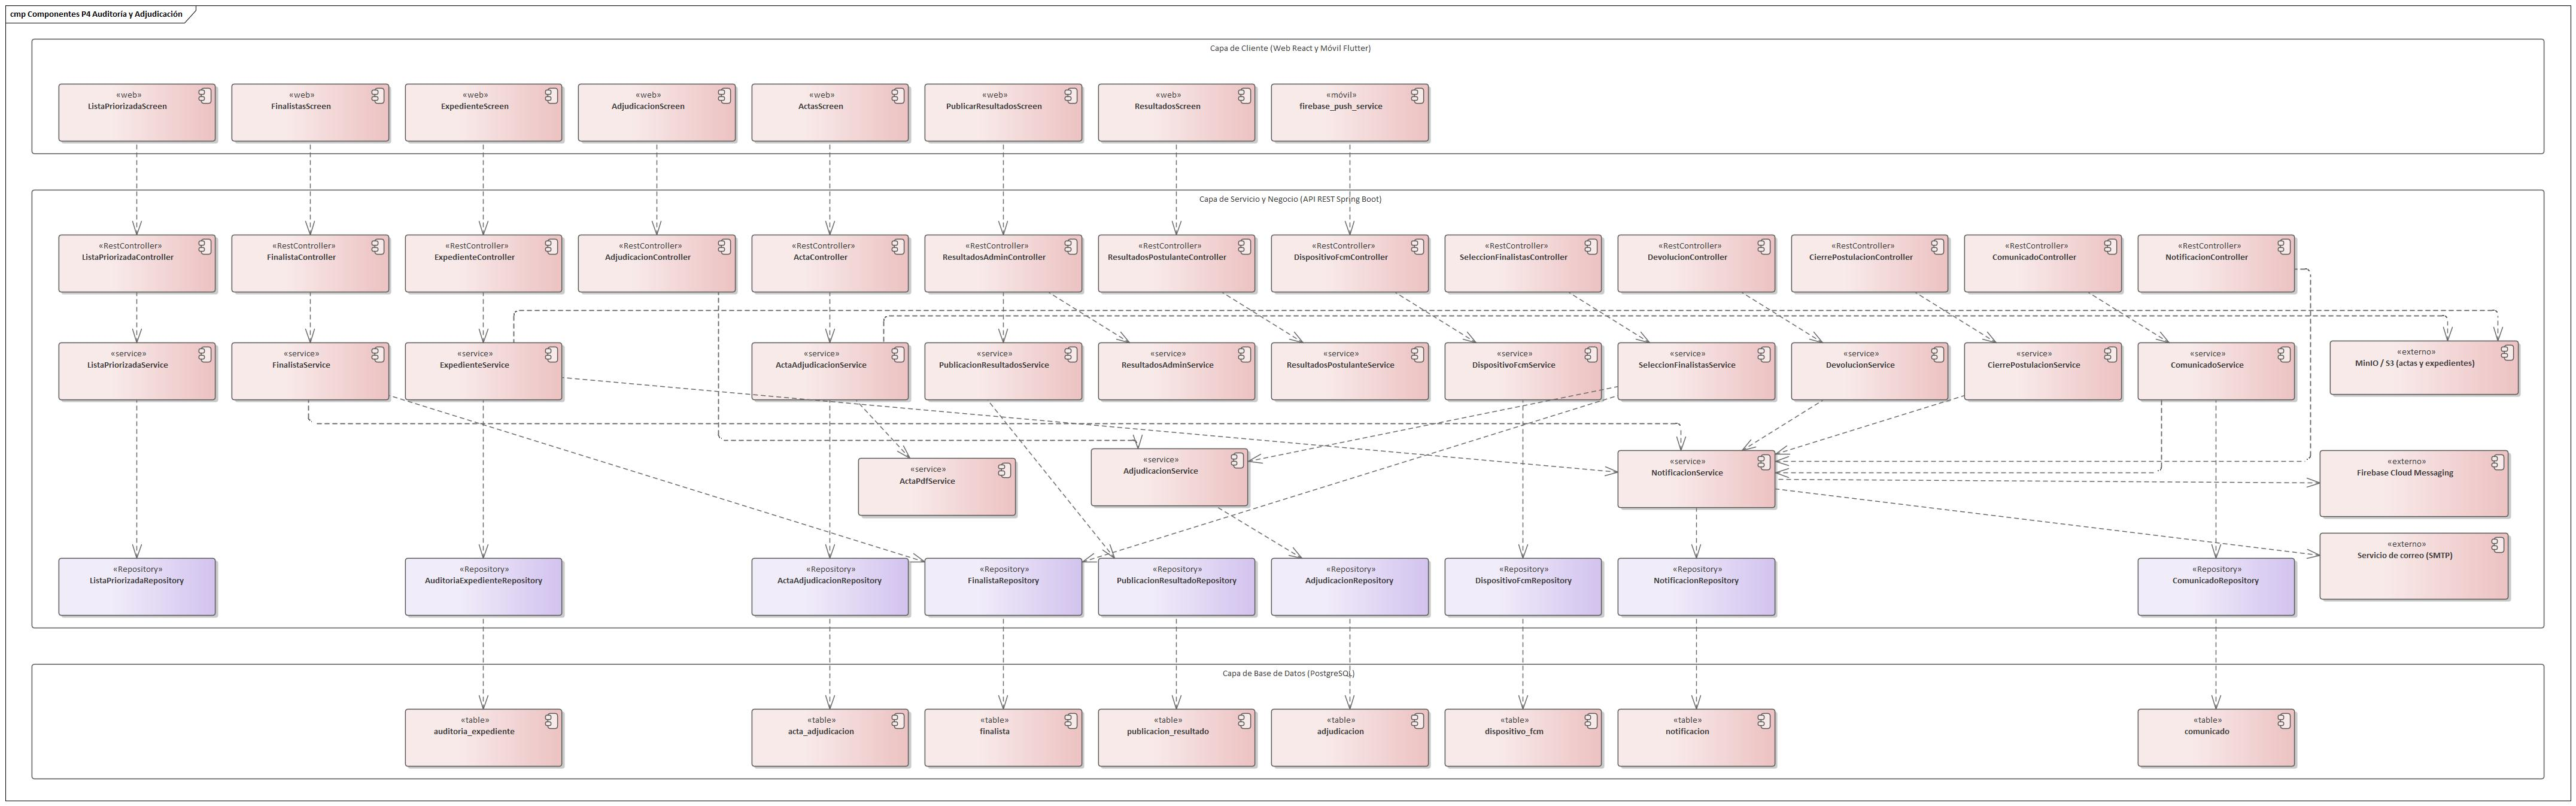
\includegraphics[width=\linewidth,height=0.8\textheight,keepaspectratio]{images/151_Componentes_P4_Auditoria_y_Adjudicacion.jpg}

\smallskip
\noindent\raggedright\textit{Nota.} Elaboración propia.
\end{figure}
\end{landscape}


\wfb{\wn{8}.2.5. Implementación de la Arquitectura del Subsistema Becados y Asistencia}\label{sec:cap8_sub_p5}

Este subsistema agrupa los casos de uso CU23, CU09, CU10, CU11, CU24.

Administra el padrón de becados (alta, baja, suspensión y reemplazo), genera las planillas de asistencia en PDF, registra la asistencia digital desde la app móvil del personal del comedor, coteja el registro contra el respaldo físico y permite al becado consultar su historial de asistencia y el estado de su beca.

La Figura~\ref{fig:impl_p5} presenta el diagrama de componentes del subsistema. Sus componentes son los siguientes:

\begin{itemize}
\item \textbf{Cliente web:} \texttt{PadronScreen}, \texttt{PlanillasScreen}, \texttt{CotejoScreen}, \texttt{MiBecaScreen}.
\item \textbf{Cliente móvil:} \texttt{registrar\_asistencia\_screen}, \texttt{mibeca (mi\_beca\_vista)}.
\item \textbf{Controladores:} \texttt{PadronController}, \texttt{BecaController}, \texttt{PlanillaController}, \texttt{AsistenciaController}, \texttt{CotejoController}, \texttt{MiBecaController}.
\item \textbf{Servicios:} \texttt{PadronService}, \texttt{BecaEstadoService}, \texttt{PlanillaAsistenciaService}, \texttt{PlanillaPdfService}, \texttt{AsistenciaService}, \texttt{CotejoAsistenciaService}, \texttt{MiBecaService}.
\item \textbf{Repositorios:} \texttt{BecaRepository}, \texttt{MovimientoBecaRepository}, \texttt{PlanillaAsistenciaRepository}, \texttt{AsistenciaRepository}, \texttt{CotejoAsistenciaRepository}, \texttt{MiBecaConsultaRepository}.
\item \textbf{Tablas:} \texttt{beca}, \texttt{movimiento\_beca}, \texttt{planilla\_asistencia}, \texttt{asistencia}, \texttt{cotejo\_asistencia}.
\item \textbf{Componentes externos:} MinIO (planillas PDF).
\end{itemize}

\begin{landscape}
\begin{figure}[p]
\caption{Diagrama de Componentes de la Implementación de la Arquitectura del Subsistema Becados y Asistencia}
\label{fig:impl_p5}
\centering
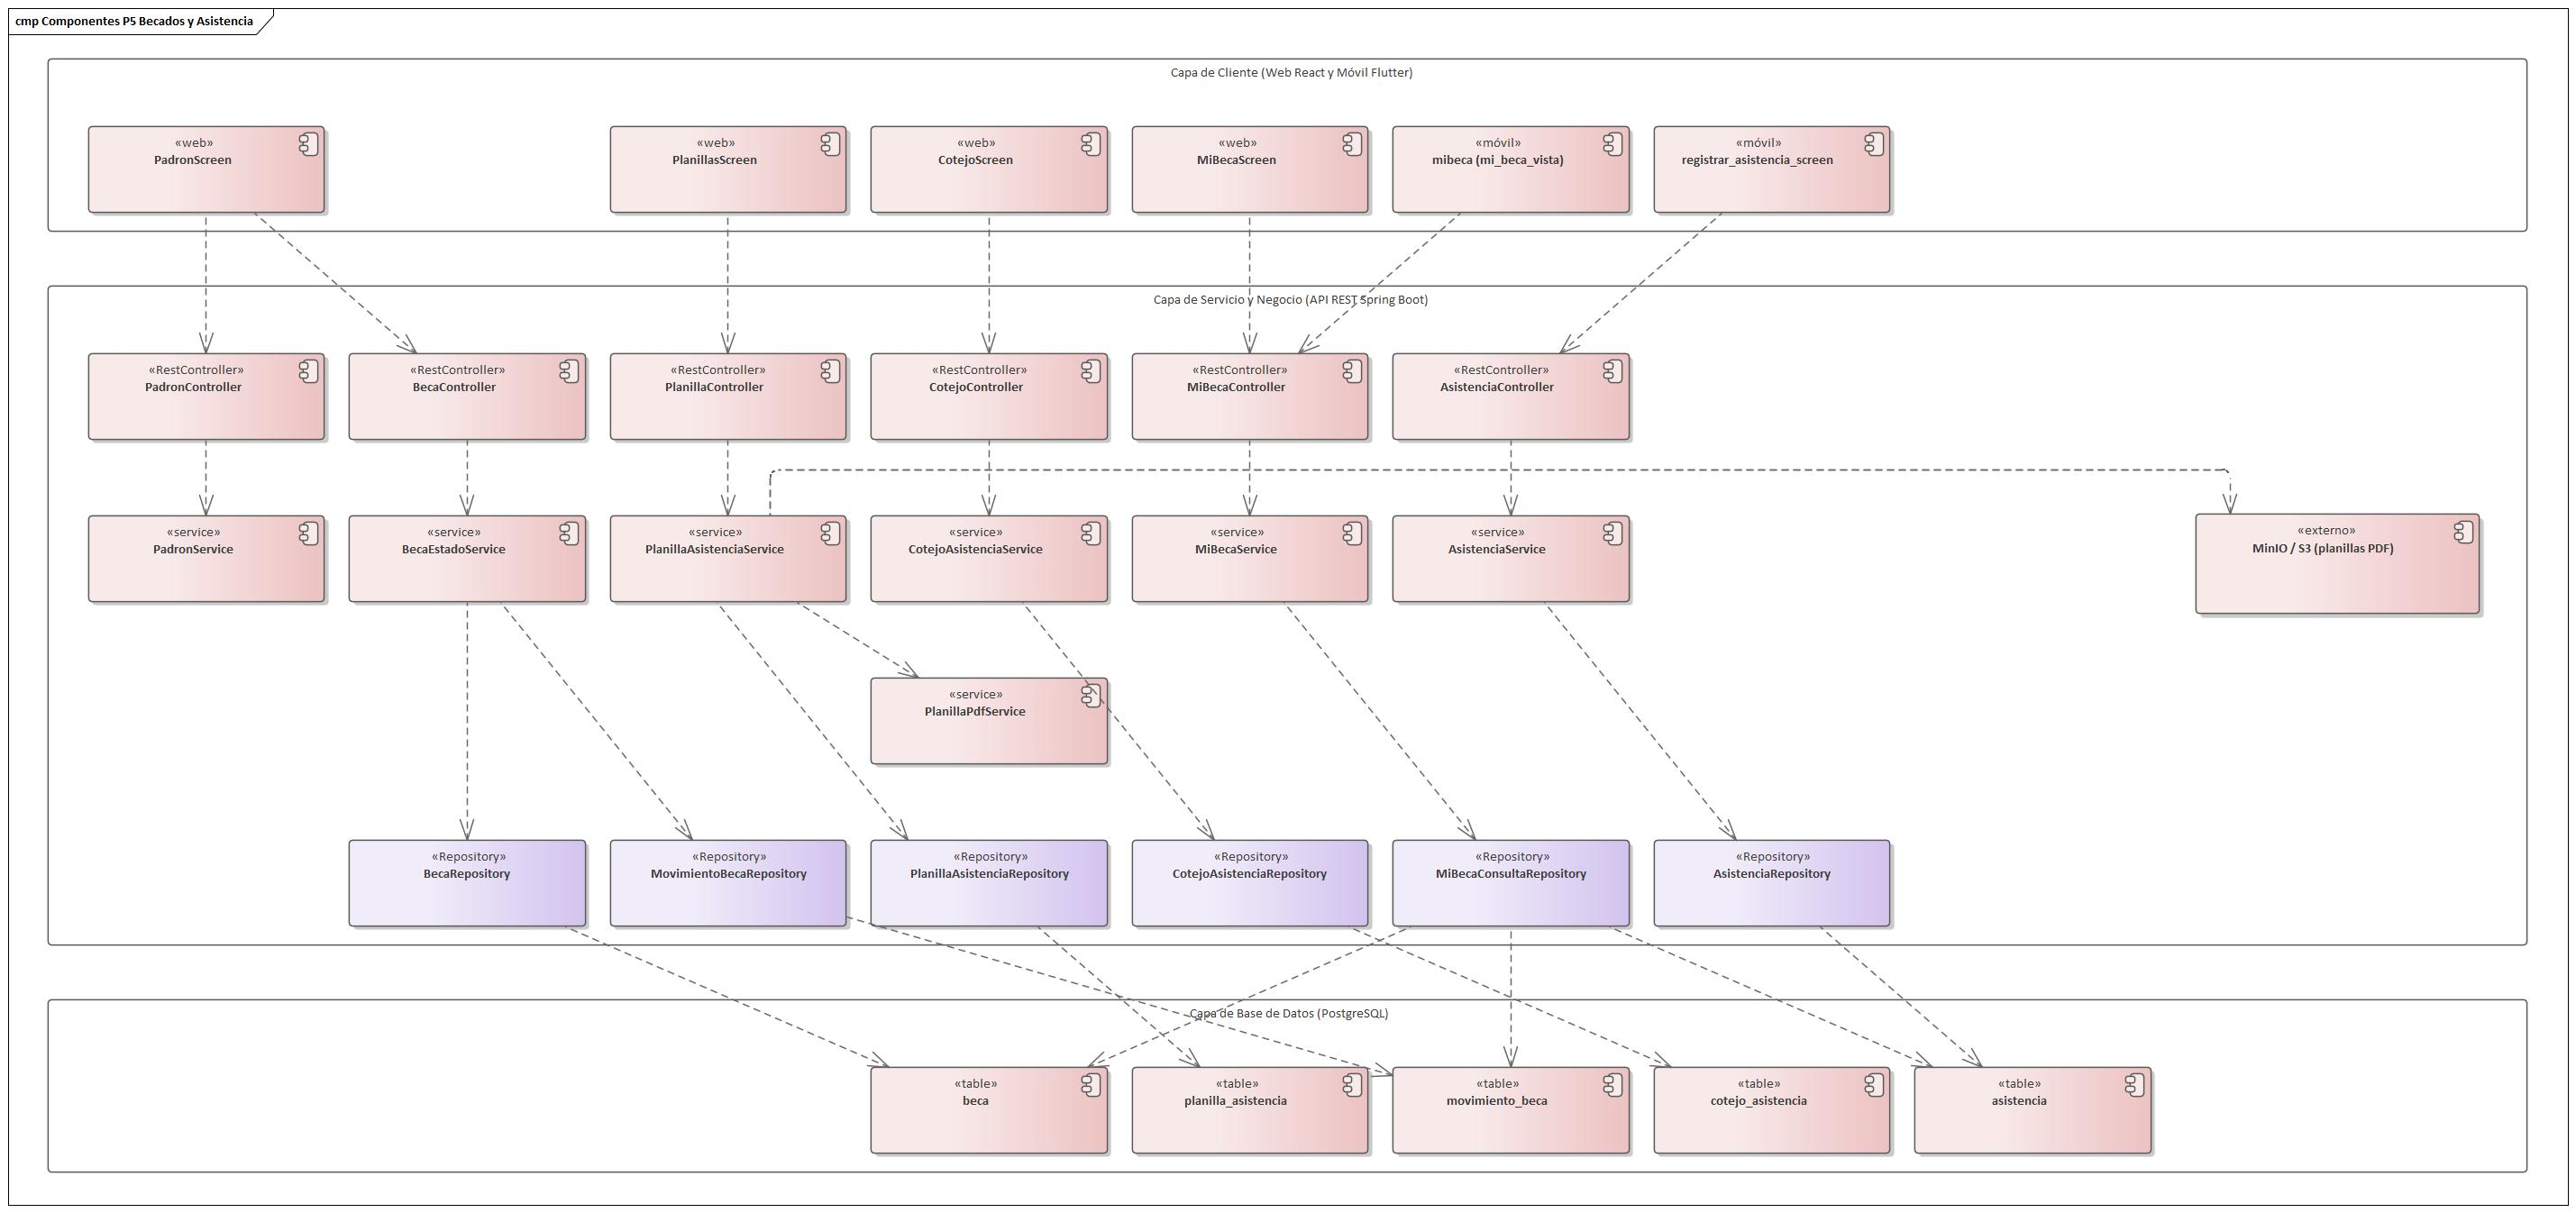
\includegraphics[width=\linewidth,height=0.8\textheight,keepaspectratio]{images/152_Componentes_P5_Becados_y_Asistencia.jpg}

\smallskip
\noindent\raggedright\textit{Nota.} Elaboración propia.
\end{figure}
\end{landscape}


\wfb{\wn{8}.2.6. Implementación de la Arquitectura del Subsistema Reportes y Trazabilidad}\label{sec:cap8_sub_p6}

Este subsistema agrupa los casos de uso CU12, CU25.

Ofrece el tablero de indicadores BI para el directivo (con exportación a Excel y PDF y caché en Redis), la bitácora de acciones del sistema y los paneles de inicio por rol. Los indicadores se leen de cinco vistas materializadas de PostgreSQL que \texttt{RefrescoIndicadoresJob} y \texttt{RefrescoIndicadoresService} actualizan; la bitácora se escribe desde cualquier servicio mediante la anotación \texttt{@Auditar} (\texttt{AuditoriaAspect}).

La Figura~\ref{fig:impl_p6} presenta el diagrama de componentes del subsistema. Sus componentes son los siguientes:

\begin{itemize}
\item \textbf{Cliente web:} \texttt{DashboardScreen}, \texttt{BitacoraScreen}, \texttt{PanelAdministradorScreen}.
\item \textbf{Controladores:} \texttt{DashboardController}, \texttt{BitacoraController}, \texttt{PanelController}.
\item \textbf{Servicios:} \texttt{IndicadoresService}, \texttt{BiService}, \texttt{FiltrosDashboardService}, \texttt{BiExcelService}, \texttt{IndicadoresPdfService}, \texttt{RefrescoIndicadoresJob}, \texttt{BitacoraService}, \texttt{BitacoraConsultaService}, \texttt{PanelService}.
\item \textbf{Repositorios:} \texttt{IndicadoresRepository}, \texttt{BiRepository}, \texttt{FiltrosDashboardRepository}, \texttt{BitacoraRepository}, \texttt{PanelRepository}.
\item \textbf{Tablas:} \texttt{mv\_bi\_asistencia\_dia}, \texttt{mv\_indicadores\_convocatoria}, \texttt{mv\_bi\_carrera\_convocatoria}, \texttt{mv\_bi\_convocatoria}, \texttt{mv\_bi\_puntaje\_convocatoria}, \texttt{bitacora}.
\item \textbf{Componentes externos:} Redis (caché del dashboard BI, CU12).
\end{itemize}

\begin{landscape}
\begin{figure}[p]
\caption{Diagrama de Componentes de la Implementación de la Arquitectura del Subsistema Reportes y Trazabilidad}
\label{fig:impl_p6}
\centering
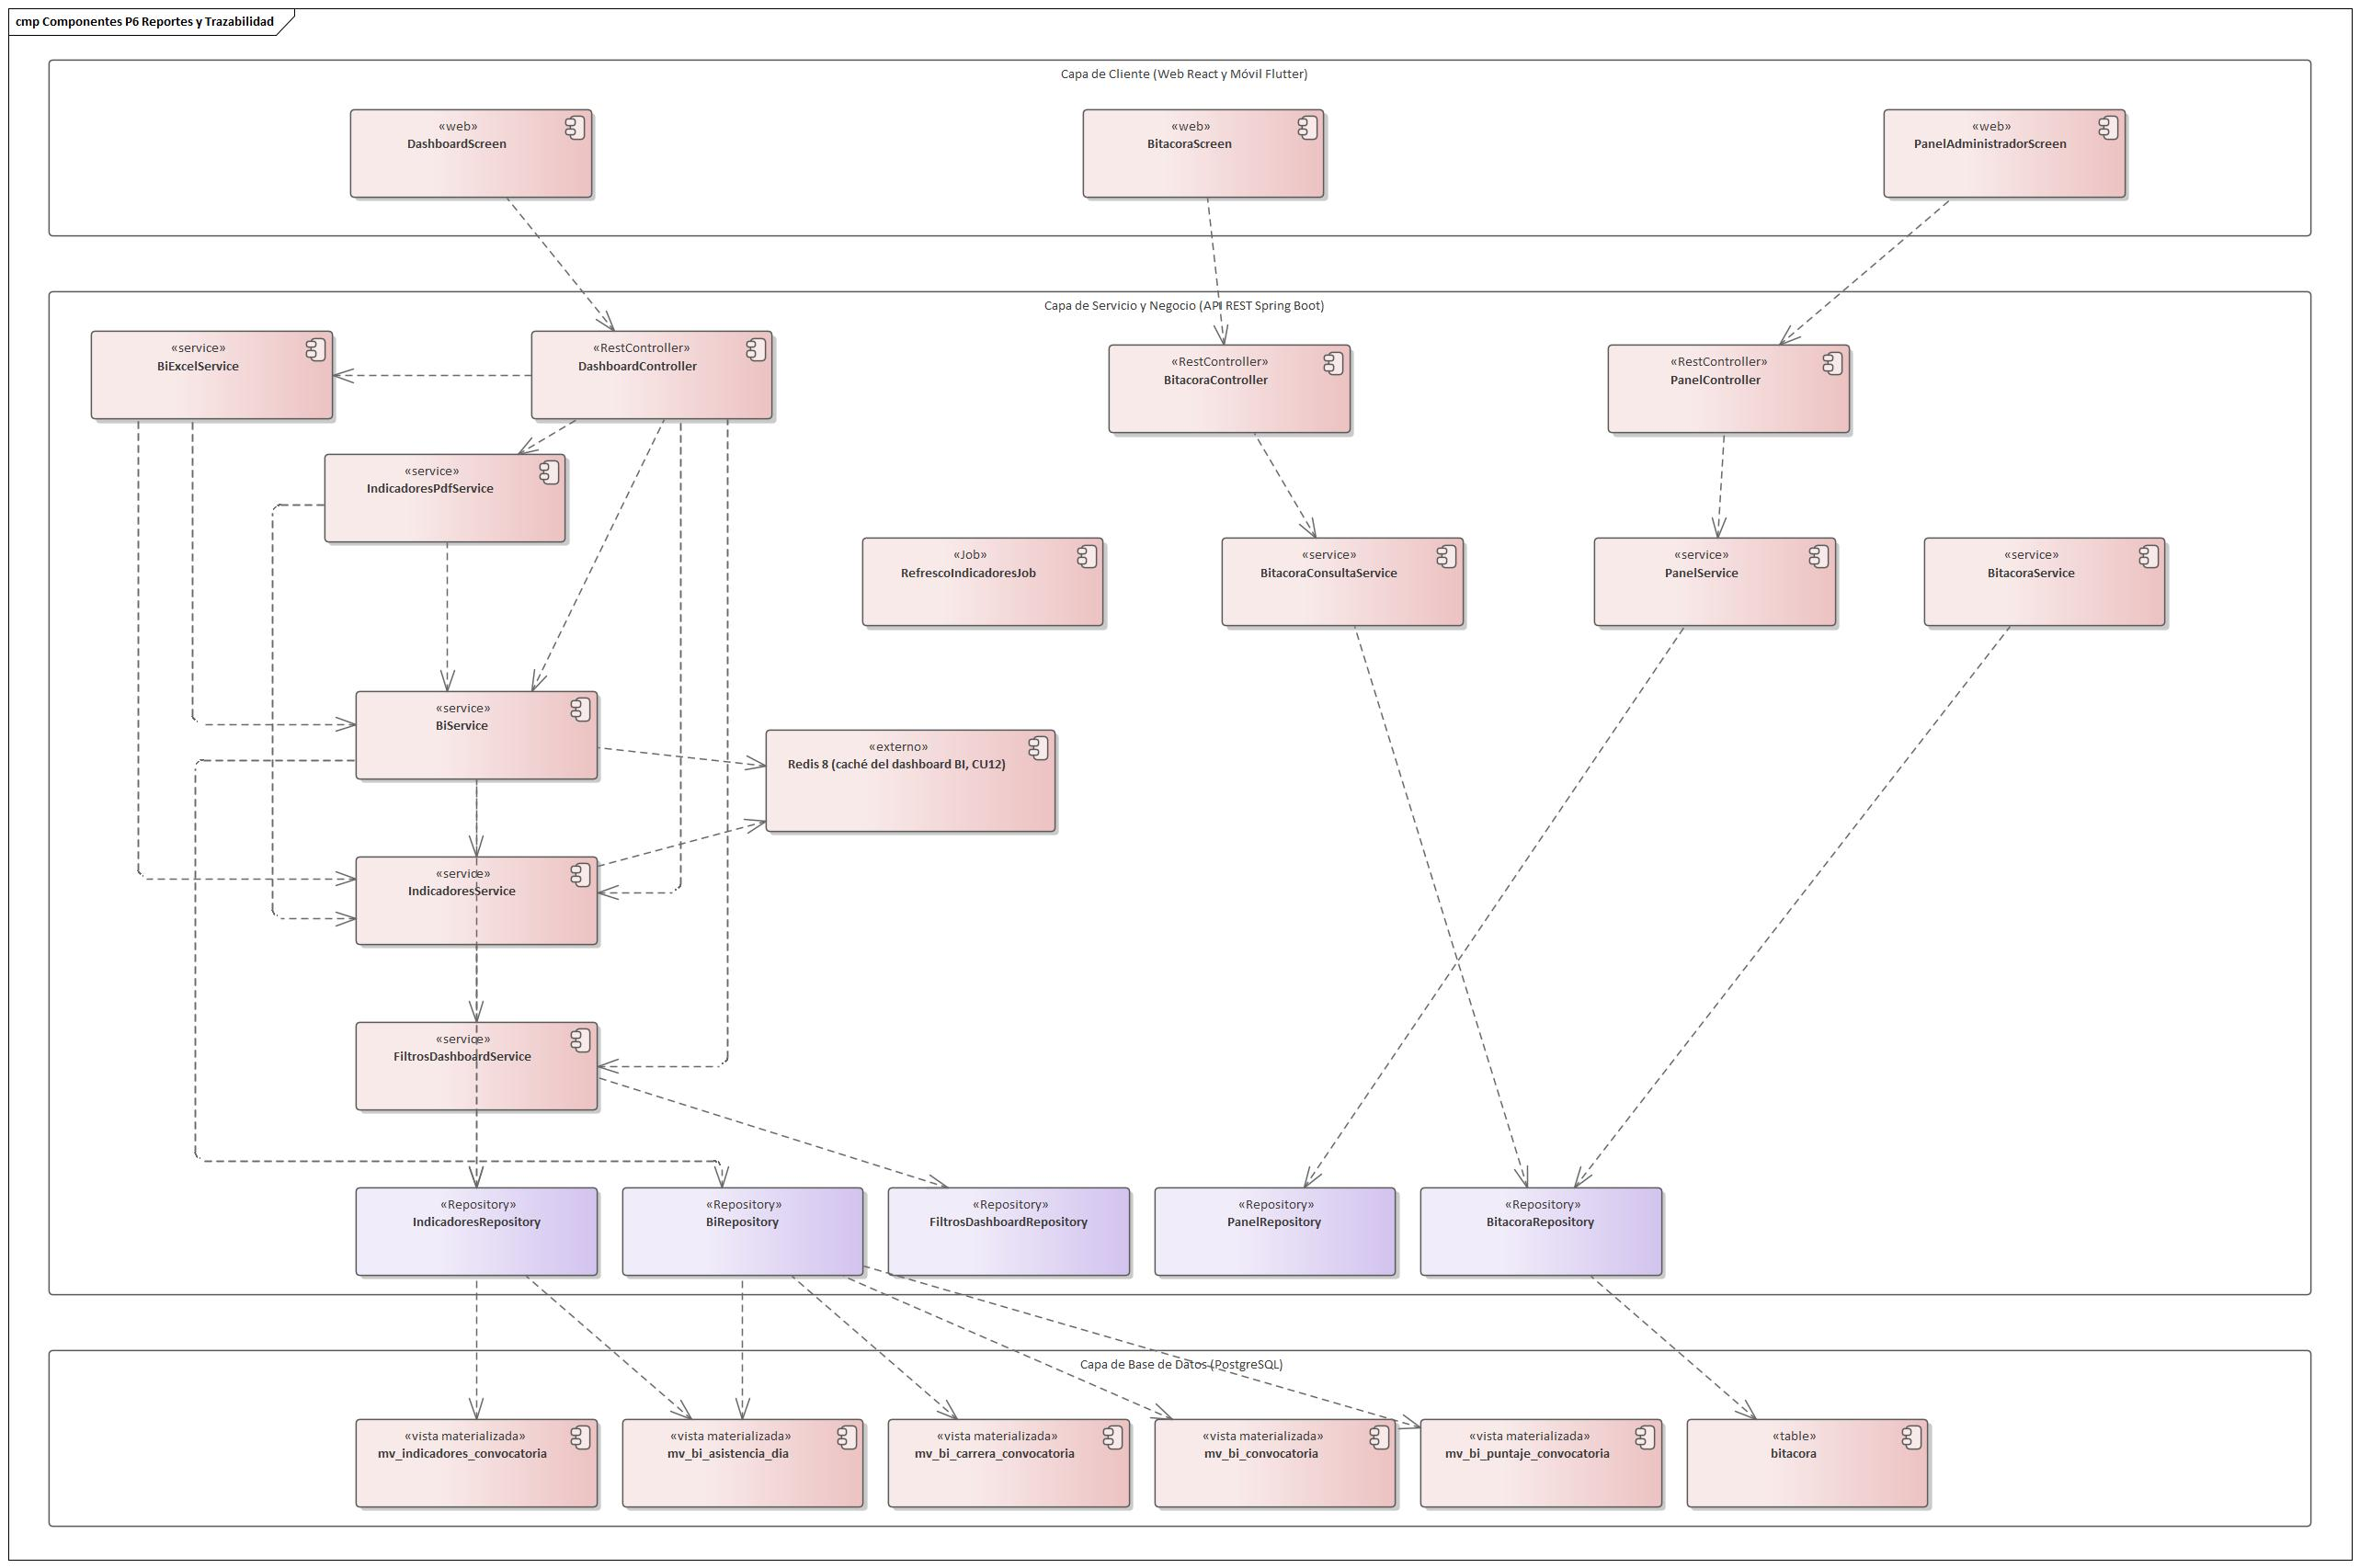
\includegraphics[width=\linewidth,height=0.8\textheight,keepaspectratio]{images/153_Componentes_P6_Reportes_y_Trazabilidad.jpg}

\smallskip
\noindent\raggedright\textit{Nota.} Elaboración propia.
\end{figure}
\end{landscape}


% ------------------------------------------------------------------------------
% 8.3. HERRAMIENTAS PARA EL DESARROLLO
% ------------------------------------------------------------------------------
\subsection{8.3. Herramientas para el Desarrollo}\label{sec:cap8_herramientas}

Las versiones citadas se tomaron de los archivos de dependencias del proyecto (\texttt{pom.xml}, \texttt{package.json}, \texttt{pubspec.yaml}, \texttt{requirements.txt}) y de \texttt{docker-compose.yml}. En el panel web y en la aplicación móvil figura el rango de versión declarado.

\subsubsection{8.3.1. Lenguajes de programación}\label{sec:cap8_lenguajes}

\begin{table}[H]
\caption{Lenguajes de programación utilizados}
\label{tab:impl_lenguajes}
\centering
\footnotesize\linespread{1}\selectfont
\renewcommand{\arraystretch}{1.3}
\begin{tabular}{>{\raggedright\arraybackslash}p{3.5cm}>{\raggedright\arraybackslash}p{2.5cm}>{\raggedright\arraybackslash}p{9cm}}
\toprule
\textbf{Lenguaje} & \textbf{Versión} & \textbf{Uso} \\
\midrule
Java & 21 & API REST \texttt{comedor-uagrm-core} \\
TypeScript & 6.0 & Panel web (React) y landing (Astro) \\
Dart & SDK 3.12 & Aplicación móvil \\
Python & 3.12 & Módulo de IA \texttt{comedor-uagrm-ia} \\
SQL (PostgreSQL) & 18 & Migraciones Flyway, vistas materializadas y consultas \\
HTML y CSS & --- & Interfaces web (CSS con Tailwind) \\
\bottomrule
\end{tabular}

\smallskip
\noindent\raggedright\textit{Nota.} Elaboración propia.
\end{table}

\subsubsection{8.3.2. Librerías}\label{sec:cap8_librerias}

La Tabla~\ref{tab:impl_librerias_back} lista las librerías del \textit{backend}. Las que figuran como BOM toman la versión de Spring Boot 4.1.2.

\begin{table}[H]
\caption{Librerías del backend (Java, Maven)}
\label{tab:impl_librerias_back}
\centering
\footnotesize\linespread{1}\selectfont
\renewcommand{\arraystretch}{1.3}
\begin{tabular}{>{\raggedright\arraybackslash}p{5.5cm}>{\raggedright\arraybackslash}p{2cm}>{\raggedright\arraybackslash}p{7.5cm}}
\toprule
\textbf{Librería} & \textbf{Versión} & \textbf{Propósito} \\
\midrule
Spring Security y OAuth2 Resource Server & BOM & Verificación del JWT y control de acceso por rol \\
Spring Data JPA (Hibernate) & BOM & Persistencia \\
Flyway & BOM & Migraciones de la base de datos \\
Spring Validation, Mail y AOP (AspectJ) & BOM & Validación, correo y auditoría con \texttt{@Auditar} \\
Actuator y Micrometer Prometheus & BOM & Métricas y estado de salud \\
springdoc-openapi & 2.8.5 & Documentación OpenAPI y Swagger UI \\
MinIO Java client & 8.5.17 & Archivos en MinIO (S3) \\
Bucket4j & 8.14.0 & Límite de peticiones por IP \\
JasperReports & 7.1.0 & PDF de lista priorizada, actas y planillas \\
Apache POI & 5.4.1 & Exportación a Excel \\
Firebase Admin SDK & 9.11.0 & Notificaciones \textit{push} (FCM) \\
logstash-logback-encoder & 8.1 & Registros (\textit{logs}) en JSON \\
Spring Data Redis & BOM & Caché del dashboard BI (CU12) \\
Lombok & BOM & Reducción de código repetitivo \\
Testcontainers & 1.21.3 & Pruebas con PostgreSQL real \\
Checkstyle (plugin) & 3.6.0 & Estilo de código \\
\bottomrule
\end{tabular}

\smallskip
\noindent\raggedright\textit{Nota.} Elaboración propia.
\end{table}

Las Tablas~\ref{tab:impl_librerias_web}, \ref{tab:impl_librerias_movil} y \ref{tab:impl_librerias_otros} presentan las librerías del panel web, de la aplicación móvil, del módulo de IA y de la landing de Nexware.

\begin{table}[H]
\caption{Librerías del panel web (React, pnpm)}
\label{tab:impl_librerias_web}
\centering
\footnotesize\linespread{1}\selectfont
\renewcommand{\arraystretch}{1.3}
\begin{tabular}{>{\raggedright\arraybackslash}p{4.5cm}>{\raggedright\arraybackslash}p{2.5cm}>{\raggedright\arraybackslash}p{8cm}}
\toprule
\textbf{Librería} & \textbf{Versión} & \textbf{Propósito} \\
\midrule
TanStack Query & 5.101 & Consulta y caché de datos del servidor \\
TanStack Router & 1.170 & Rutas y navegación \\
TanStack Form & 1.33 & Formularios \\
TanStack Table & 8.21 & Tablas de datos con paginación \\
Zustand & 5.0 & Estado de la interfaz \\
Zod & 4.4 & Validación de formularios y datos \\
Axios & 1.19 & Cliente HTTP \\
Recharts & 3.8 & Gráficos del dashboard \\
shadcn & 4.16 & Componentes de interfaz \\
Base UI & 1.6 & Componentes base accesibles \\
Vitest y Testing Library & 4.1 y 16.3 & Pruebas unitarias y de componentes \\
ESLint y Prettier & 10 y 3.9 & Análisis y formato del código \\
\bottomrule
\end{tabular}

\smallskip
\noindent\raggedright\textit{Nota.} Elaboración propia.
\end{table}

\begin{table}[H]
\caption{Librerías de la aplicación móvil (Flutter)}
\label{tab:impl_librerias_movil}
\centering
\footnotesize\linespread{1}\selectfont
\renewcommand{\arraystretch}{1.3}
\begin{tabular}{>{\raggedright\arraybackslash}p{4.5cm}>{\raggedright\arraybackslash}p{2.5cm}>{\raggedright\arraybackslash}p{8cm}}
\toprule
\textbf{Librería} & \textbf{Versión} & \textbf{Propósito} \\
\midrule
flutter\_riverpod & 2.6 & Estado de la aplicación \\
go\_router & 18.0 & Navegación \\
dio & 5.11 & Cliente HTTP \\
flutter\_secure\_storage & 10.3 & Almacenamiento seguro del \textit{refresh token} \\
firebase\_core & 5.1 & Inicialización de Firebase \\
firebase\_messaging & 17.0 & Notificaciones \textit{push} \\
image\_picker & 1.2 & Captura de fotos con la cámara \\
image\_cropper & 12.2 & Recorte de imágenes de documentos \\
file\_picker & 13.3 & Selección de archivos a adjuntar \\
flutter\_lints & 6.0 & Análisis estático del código \\
\bottomrule
\end{tabular}

\smallskip
\noindent\raggedright\textit{Nota.} Elaboración propia.
\end{table}

\begin{table}[H]
\caption{Librerías del módulo de IA (Python) y de la landing de Nexware (Astro)}
\label{tab:impl_librerias_otros}
\centering
\footnotesize\linespread{1}\selectfont
\renewcommand{\arraystretch}{1.3}
\begin{tabular}{>{\raggedright\arraybackslash}p{4.5cm}>{\raggedright\arraybackslash}p{2.5cm}>{\raggedright\arraybackslash}p{8cm}}
\toprule
\textbf{Librería} & \textbf{Versión} & \textbf{Propósito} \\
\midrule
scikit-learn & 1.9.1 & Modelo de aprendizaje automático (segunda opinión) \\
NumPy & 2.3.3 & Cálculo numérico \\
joblib & 1.6.0 & Carga del modelo entrenado \\
Uvicorn & 0.54.0 & Servidor ASGI del módulo de IA \\
\texttt{@astrojs/sitemap} & 3.7 & Mapa del sitio de la landing \\
\texttt{sharp} & 0.35 & Optimización de imágenes de la landing \\
Space Grotesk y JetBrains Mono & --- & Tipografías de la landing (\texttt{@fontsource}) \\
Vitest & 5.0 & Pruebas de la landing \\
\bottomrule
\end{tabular}

\smallskip
\noindent\raggedright\textit{Nota.} Elaboración propia.
\end{table}

\subsubsection{8.3.3. Frameworks}\label{sec:cap8_frameworks}

\begin{table}[H]
\caption{Frameworks utilizados}
\label{tab:impl_frameworks}
\centering
\footnotesize\linespread{1}\selectfont
\renewcommand{\arraystretch}{1.3}
\begin{tabular}{>{\raggedright\arraybackslash}p{3.5cm}>{\raggedright\arraybackslash}p{2.5cm}>{\raggedright\arraybackslash}p{9cm}}
\toprule
\textbf{Framework} & \textbf{Versión} & \textbf{Uso} \\
\midrule
Spring Boot & 4.1.2 & API REST (con Spring MVC, Security y Data JPA) \\
React & 19.2 & Panel web \\
Vite & 8.2 & Servidor de desarrollo y empaquetado del panel \\
Tailwind CSS & 4.0 & Estilos del panel web \\
Astro & 7.4 & Landing institucional estática (español e inglés) \\
Flutter & Dart 3.12 & Aplicación móvil Android \\
FastAPI & 0.162.0 & Módulo de IA \\
Docker Compose & --- & Orquestación del entorno: nginx, core, ia, panel, landing, postgres, redis, minio, mailpit, prometheus y grafana \\
\bottomrule
\end{tabular}

\smallskip
\noindent\raggedright\textit{Nota.} Elaboración propia.
\end{table}

\subsubsection{8.3.4. Sistema gestor de base de datos}\label{sec:cap8_sgbd}

El sistema gestor de base de datos es PostgreSQL 18 (imagen \texttt{postgres:18-alpine}), al que la API accede por JDBC. El esquema se gestiona con migraciones Flyway versionadas por fecha y hora (\texttt{V\{aaaaMMddHHmmss\}\_\_descripcion.sql}; 25 migraciones al redactar este capítulo). Cada tabla tiene un identificador interno \texttt{bigint} y un código público UUID, y el borrado es lógico mediante la columna \texttt{eliminado\_en}. Para el tablero BI se crearon cinco vistas materializadas. Los archivos no se guardan en la base sino en MinIO, y Redis se usa como caché del dashboard BI.

\subsubsection{8.3.5. Lenguaje de modelado de software}\label{sec:cap8_modelado}

El modelado se realizó con el Lenguaje Unificado de Modelado (UML 2.5): diagramas de casos de uso, de análisis, de secuencia, de clases, de componentes y de despliegue, elaborados con Sparx Enterprise Architect 15. El diseño lógico de la base de datos también se modeló en esa herramienta y se transcribió al archivo \texttt{DiagramaConceptual.mermaid} del repositorio del proyecto.

\subsubsection{8.3.6. Protocolo de comunicación}\label{sec:cap8_protocolos}

\begin{table}[H]
\caption{Protocolos de comunicación del sistema}
\label{tab:impl_protocolos}
\centering
\footnotesize\linespread{1}\selectfont
\renewcommand{\arraystretch}{1.3}
\begin{tabular}{>{\raggedright\arraybackslash}p{5cm}>{\raggedright\arraybackslash}p{10cm}}
\toprule
\textbf{Enlace} & \textbf{Protocolo y formato} \\
\midrule
Navegador o app móvil con la API & HTTP (HTTPS en producción), arquitectura REST con JSON bajo \texttt{/api/v1}; carga de archivos con \texttt{multipart/form-data} \\
Autenticación & JWT (HS256): cookies \texttt{HttpOnly} en la web y cabecera \texttt{Authorization: Bearer} en móvil \\
API con el módulo de IA & HTTP interno con JSON (\texttt{POST /api/v1/puntaje}) en la red de Docker \\
API con PostgreSQL & JDBC sobre el protocolo de PostgreSQL \\
API con MinIO & API compatible con S3 sobre HTTP \\
API con Redis & RESP sobre TCP (caché del dashboard, CU12) \\
API con el correo & SMTP (Mailpit en desarrollo) \\
API con Firebase & Firebase Admin SDK hacia FCM (HTTPS) \\
Prometheus con la API & HTTP, punto de acceso \texttt{/prometheus} \\
\bottomrule
\end{tabular}

\smallskip
\noindent\raggedright\textit{Nota.} Elaboración propia.
\end{table}


